\documentclass[a4paper]{article}

% if you need to pass options to natbib, use, e.g.:
%     \PassOptionsToPackage{numbers, compress}{natbib}
% before loading neurips_2022


% ready for submission
%\usepackage{ofu_xai_2022}

% SOURCE: https://github.com/goodfeli/dlbook_notation/blob/master/math_commands.tex
% Quote from github "We make them freely available for anyone to use."

\usepackage{amsmath,amsfonts,bm}


%%%%% NEW MATH DEFINITIONS %%%%%

% Mark sections of captions for referring to divisions of figures
\newcommand{\figleft}{{\em (Left)}}
\newcommand{\figcenter}{{\em (Center)}}
\newcommand{\figright}{{\em (Right)}}
\newcommand{\figtop}{{\em (Top)}}
\newcommand{\figbottom}{{\em (Bottom)}}
\newcommand{\captiona}{{\em (a)}}
\newcommand{\captionb}{{\em (b)}}
\newcommand{\captionc}{{\em (c)}}
\newcommand{\captiond}{{\em (d)}}

% Highlight a newly defined term
\newcommand{\newterm}[1]{{\bf #1}}


% Figure reference, lower-case.
\def\figref#1{figure~\ref{#1}}
% Figure reference, capital. For start of sentence
\def\Figref#1{Figure~\ref{#1}}
\def\twofigref#1#2{figures \ref{#1} and \ref{#2}}
\def\quadfigref#1#2#3#4{figures \ref{#1}, \ref{#2}, \ref{#3} and \ref{#4}}
% Section reference, lower-case.
\def\secref#1{section~\ref{#1}}
% Section reference, capital.
\def\Secref#1{Section~\ref{#1}}
% Reference to two sections.
\def\twosecrefs#1#2{sections \ref{#1} and \ref{#2}}
% Reference to three sections.
\def\secrefs#1#2#3{sections \ref{#1}, \ref{#2} and \ref{#3}}
% Reference to an equation, lower-case.
\def\eqref#1{equation~\ref{#1}}
% Reference to an equation, upper case
\def\Eqref#1{Equation~\ref{#1}}
% A raw reference to an equation---avoid using if possible
\def\plaineqref#1{\ref{#1}}
% Reference to a chapter, lower-case.
\def\chapref#1{chapter~\ref{#1}}
% Reference to an equation, upper case.
\def\Chapref#1{Chapter~\ref{#1}}
% Reference to a range of chapters
\def\rangechapref#1#2{chapters\ref{#1}--\ref{#2}}
% Reference to an algorithm, lower-case.
\def\algref#1{algorithm~\ref{#1}}
% Reference to an algorithm, upper case.
\def\Algref#1{Algorithm~\ref{#1}}
\def\twoalgref#1#2{algorithms \ref{#1} and \ref{#2}}
\def\Twoalgref#1#2{Algorithms \ref{#1} and \ref{#2}}
% Reference to a part, lower case
\def\partref#1{part~\ref{#1}}
% Reference to a part, upper case
\def\Partref#1{Part~\ref{#1}}
\def\twopartref#1#2{parts \ref{#1} and \ref{#2}}

\def\ceil#1{\lceil #1 \rceil}
\def\floor#1{\lfloor #1 \rfloor}
\def\1{\bm{1}}
\newcommand{\train}{\mathcal{D}}
\newcommand{\valid}{\mathcal{D_{\mathrm{valid}}}}
\newcommand{\test}{\mathcal{D_{\mathrm{test}}}}

\def\eps{{\epsilon}}


% Random variables
\def\reta{{\textnormal{$\eta$}}}
\def\ra{{\textnormal{a}}}
\def\rb{{\textnormal{b}}}
\def\rc{{\textnormal{c}}}
\def\rd{{\textnormal{d}}}
\def\re{{\textnormal{e}}}
\def\rf{{\textnormal{f}}}
\def\rg{{\textnormal{g}}}
\def\rh{{\textnormal{h}}}
\def\ri{{\textnormal{i}}}
\def\rj{{\textnormal{j}}}
\def\rk{{\textnormal{k}}}
\def\rl{{\textnormal{l}}}
% rm is already a command, just don't name any random variables m
\def\rn{{\textnormal{n}}}
\def\ro{{\textnormal{o}}}
\def\rp{{\textnormal{p}}}
\def\rq{{\textnormal{q}}}
\def\rr{{\textnormal{r}}}
\def\rs{{\textnormal{s}}}
\def\rt{{\textnormal{t}}}
\def\ru{{\textnormal{u}}}
\def\rv{{\textnormal{v}}}
\def\rw{{\textnormal{w}}}
\def\rx{{\textnormal{x}}}
\def\ry{{\textnormal{y}}}
\def\rz{{\textnormal{z}}}

% Random vectors
\def\rvepsilon{{\mathbf{\epsilon}}}
\def\rvtheta{{\mathbf{\theta}}}
\def\rva{{\mathbf{a}}}
\def\rvb{{\mathbf{b}}}
\def\rvc{{\mathbf{c}}}
\def\rvd{{\mathbf{d}}}
\def\rve{{\mathbf{e}}}
\def\rvf{{\mathbf{f}}}
\def\rvg{{\mathbf{g}}}
\def\rvh{{\mathbf{h}}}
\def\rvu{{\mathbf{i}}}
\def\rvj{{\mathbf{j}}}
\def\rvk{{\mathbf{k}}}
\def\rvl{{\mathbf{l}}}
\def\rvm{{\mathbf{m}}}
\def\rvn{{\mathbf{n}}}
\def\rvo{{\mathbf{o}}}
\def\rvp{{\mathbf{p}}}
\def\rvq{{\mathbf{q}}}
\def\rvr{{\mathbf{r}}}
\def\rvs{{\mathbf{s}}}
\def\rvt{{\mathbf{t}}}
\def\rvu{{\mathbf{u}}}
\def\rvv{{\mathbf{v}}}
\def\rvw{{\mathbf{w}}}
\def\rvx{{\mathbf{x}}}
\def\rvy{{\mathbf{y}}}
\def\rvz{{\mathbf{z}}}

% Elements of random vectors
\def\erva{{\textnormal{a}}}
\def\ervb{{\textnormal{b}}}
\def\ervc{{\textnormal{c}}}
\def\ervd{{\textnormal{d}}}
\def\erve{{\textnormal{e}}}
\def\ervf{{\textnormal{f}}}
\def\ervg{{\textnormal{g}}}
\def\ervh{{\textnormal{h}}}
\def\ervi{{\textnormal{i}}}
\def\ervj{{\textnormal{j}}}
\def\ervk{{\textnormal{k}}}
\def\ervl{{\textnormal{l}}}
\def\ervm{{\textnormal{m}}}
\def\ervn{{\textnormal{n}}}
\def\ervo{{\textnormal{o}}}
\def\ervp{{\textnormal{p}}}
\def\ervq{{\textnormal{q}}}
\def\ervr{{\textnormal{r}}}
\def\ervs{{\textnormal{s}}}
\def\ervt{{\textnormal{t}}}
\def\ervu{{\textnormal{u}}}
\def\ervv{{\textnormal{v}}}
\def\ervw{{\textnormal{w}}}
\def\ervx{{\textnormal{x}}}
\def\ervy{{\textnormal{y}}}
\def\ervz{{\textnormal{z}}}

% Random matrices
\def\rmA{{\mathbf{A}}}
\def\rmB{{\mathbf{B}}}
\def\rmC{{\mathbf{C}}}
\def\rmD{{\mathbf{D}}}
\def\rmE{{\mathbf{E}}}
\def\rmF{{\mathbf{F}}}
\def\rmG{{\mathbf{G}}}
\def\rmH{{\mathbf{H}}}
\def\rmI{{\mathbf{I}}}
\def\rmJ{{\mathbf{J}}}
\def\rmK{{\mathbf{K}}}
\def\rmL{{\mathbf{L}}}
\def\rmM{{\mathbf{M}}}
\def\rmN{{\mathbf{N}}}
\def\rmO{{\mathbf{O}}}
\def\rmP{{\mathbf{P}}}
\def\rmQ{{\mathbf{Q}}}
\def\rmR{{\mathbf{R}}}
\def\rmS{{\mathbf{S}}}
\def\rmT{{\mathbf{T}}}
\def\rmU{{\mathbf{U}}}
\def\rmV{{\mathbf{V}}}
\def\rmW{{\mathbf{W}}}
\def\rmX{{\mathbf{X}}}
\def\rmY{{\mathbf{Y}}}
\def\rmZ{{\mathbf{Z}}}

% Elements of random matrices
\def\ermA{{\textnormal{A}}}
\def\ermB{{\textnormal{B}}}
\def\ermC{{\textnormal{C}}}
\def\ermD{{\textnormal{D}}}
\def\ermE{{\textnormal{E}}}
\def\ermF{{\textnormal{F}}}
\def\ermG{{\textnormal{G}}}
\def\ermH{{\textnormal{H}}}
\def\ermI{{\textnormal{I}}}
\def\ermJ{{\textnormal{J}}}
\def\ermK{{\textnormal{K}}}
\def\ermL{{\textnormal{L}}}
\def\ermM{{\textnormal{M}}}
\def\ermN{{\textnormal{N}}}
\def\ermO{{\textnormal{O}}}
\def\ermP{{\textnormal{P}}}
\def\ermQ{{\textnormal{Q}}}
\def\ermR{{\textnormal{R}}}
\def\ermS{{\textnormal{S}}}
\def\ermT{{\textnormal{T}}}
\def\ermU{{\textnormal{U}}}
\def\ermV{{\textnormal{V}}}
\def\ermW{{\textnormal{W}}}
\def\ermX{{\textnormal{X}}}
\def\ermY{{\textnormal{Y}}}
\def\ermZ{{\textnormal{Z}}}

% Vectors
\def\vzero{{\bm{0}}}
\def\vone{{\bm{1}}}
\def\vmu{{\bm{\mu}}}
\def\vtheta{{\bm{\theta}}}
\def\va{{\bm{a}}}
\def\vb{{\bm{b}}}
\def\vc{{\bm{c}}}
\def\vd{{\bm{d}}}
\def\ve{{\bm{e}}}
\def\vf{{\bm{f}}}
\def\vg{{\bm{g}}}
\def\vh{{\bm{h}}}
\def\vi{{\bm{i}}}
\def\vj{{\bm{j}}}
\def\vk{{\bm{k}}}
\def\vl{{\bm{l}}}
\def\vm{{\bm{m}}}
\def\vn{{\bm{n}}}
\def\vo{{\bm{o}}}
\def\vp{{\bm{p}}}
\def\vq{{\bm{q}}}
\def\vr{{\bm{r}}}
\def\vs{{\bm{s}}}
\def\vt{{\bm{t}}}
\def\vu{{\bm{u}}}
\def\vv{{\bm{v}}}
\def\vw{{\bm{w}}}
\def\vx{{\bm{x}}}
\def\vy{{\bm{y}}}
\def\vz{{\bm{z}}}

% Elements of vectors
\def\evalpha{{\alpha}}
\def\evbeta{{\beta}}
\def\evepsilon{{\epsilon}}
\def\evlambda{{\lambda}}
\def\evomega{{\omega}}
\def\evmu{{\mu}}
\def\evpsi{{\psi}}
\def\evsigma{{\sigma}}
\def\evtheta{{\theta}}
\def\eva{{a}}
\def\evb{{b}}
\def\evc{{c}}
\def\evd{{d}}
\def\eve{{e}}
\def\evf{{f}}
\def\evg{{g}}
\def\evh{{h}}
\def\evi{{i}}
\def\evj{{j}}
\def\evk{{k}}
\def\evl{{l}}
\def\evm{{m}}
\def\evn{{n}}
\def\evo{{o}}
\def\evp{{p}}
\def\evq{{q}}
\def\evr{{r}}
\def\evs{{s}}
\def\evt{{t}}
\def\evu{{u}}
\def\evv{{v}}
\def\evw{{w}}
\def\evx{{x}}
\def\evy{{y}}
\def\evz{{z}}

% Matrix
\def\mA{{\bm{A}}}
\def\mB{{\bm{B}}}
\def\mC{{\bm{C}}}
\def\mD{{\bm{D}}}
\def\mE{{\bm{E}}}
\def\mF{{\bm{F}}}
\def\mG{{\bm{G}}}
\def\mH{{\bm{H}}}
\def\mI{{\bm{I}}}
\def\mJ{{\bm{J}}}
\def\mK{{\bm{K}}}
\def\mL{{\bm{L}}}
\def\mM{{\bm{M}}}
\def\mN{{\bm{N}}}
\def\mO{{\bm{O}}}
\def\mP{{\bm{P}}}
\def\mQ{{\bm{Q}}}
\def\mR{{\bm{R}}}
\def\mS{{\bm{S}}}
\def\mT{{\bm{T}}}
\def\mU{{\bm{U}}}
\def\mV{{\bm{V}}}
\def\mW{{\bm{W}}}
\def\mX{{\bm{X}}}
\def\mY{{\bm{Y}}}
\def\mZ{{\bm{Z}}}
\def\mBeta{{\bm{\beta}}}
\def\mPhi{{\bm{\Phi}}}
\def\mLambda{{\bm{\Lambda}}}
\def\mSigma{{\bm{\Sigma}}}

% Tensor
\DeclareMathAlphabet{\mathsfit}{\encodingdefault}{\sfdefault}{m}{sl}
\SetMathAlphabet{\mathsfit}{bold}{\encodingdefault}{\sfdefault}{bx}{n}
\newcommand{\tens}[1]{\bm{\mathsfit{#1}}}
\def\tA{{\tens{A}}}
\def\tB{{\tens{B}}}
\def\tC{{\tens{C}}}
\def\tD{{\tens{D}}}
\def\tE{{\tens{E}}}
\def\tF{{\tens{F}}}
\def\tG{{\tens{G}}}
\def\tH{{\tens{H}}}
\def\tI{{\tens{I}}}
\def\tJ{{\tens{J}}}
\def\tK{{\tens{K}}}
\def\tL{{\tens{L}}}
\def\tM{{\tens{M}}}
\def\tN{{\tens{N}}}
\def\tO{{\tens{O}}}
\def\tP{{\tens{P}}}
\def\tQ{{\tens{Q}}}
\def\tR{{\tens{R}}}
\def\tS{{\tens{S}}}
\def\tT{{\tens{T}}}
\def\tU{{\tens{U}}}
\def\tV{{\tens{V}}}
\def\tW{{\tens{W}}}
\def\tX{{\tens{X}}}
\def\tY{{\tens{Y}}}
\def\tZ{{\tens{Z}}}


% Graph
\def\gA{{\mathcal{A}}}
\def\gB{{\mathcal{B}}}
\def\gC{{\mathcal{C}}}
\def\gD{{\mathcal{D}}}
\def\gE{{\mathcal{E}}}
\def\gF{{\mathcal{F}}}
\def\gG{{\mathcal{G}}}
\def\gH{{\mathcal{H}}}
\def\gI{{\mathcal{I}}}
\def\gJ{{\mathcal{J}}}
\def\gK{{\mathcal{K}}}
\def\gL{{\mathcal{L}}}
\def\gM{{\mathcal{M}}}
\def\gN{{\mathcal{N}}}
\def\gO{{\mathcal{O}}}
\def\gP{{\mathcal{P}}}
\def\gQ{{\mathcal{Q}}}
\def\gR{{\mathcal{R}}}
\def\gS{{\mathcal{S}}}
\def\gT{{\mathcal{T}}}
\def\gU{{\mathcal{U}}}
\def\gV{{\mathcal{V}}}
\def\gW{{\mathcal{W}}}
\def\gX{{\mathcal{X}}}
\def\gY{{\mathcal{Y}}}
\def\gZ{{\mathcal{Z}}}

% Sets
\def\sA{{\mathbb{A}}}
\def\sB{{\mathbb{B}}}
\def\sC{{\mathbb{C}}}
\def\sD{{\mathbb{D}}}
% Don't use a set called E, because this would be the same as our symbol
% for expectation.
\def\sF{{\mathbb{F}}}
\def\sG{{\mathbb{G}}}
\def\sH{{\mathbb{H}}}
\def\sI{{\mathbb{I}}}
\def\sJ{{\mathbb{J}}}
\def\sK{{\mathbb{K}}}
\def\sL{{\mathbb{L}}}
\def\sM{{\mathbb{M}}}
\def\sN{{\mathbb{N}}}
\def\sO{{\mathbb{O}}}
\def\sP{{\mathbb{P}}}
\def\sQ{{\mathbb{Q}}}
\def\sR{{\mathbb{R}}}
\def\sS{{\mathbb{S}}}
\def\sT{{\mathbb{T}}}
\def\sU{{\mathbb{U}}}
\def\sV{{\mathbb{V}}}
\def\sW{{\mathbb{W}}}
\def\sX{{\mathbb{X}}}
\def\sY{{\mathbb{Y}}}
\def\sZ{{\mathbb{Z}}}

% Entries of a matrix
\def\emLambda{{\Lambda}}
\def\emA{{A}}
\def\emB{{B}}
\def\emC{{C}}
\def\emD{{D}}
\def\emE{{E}}
\def\emF{{F}}
\def\emG{{G}}
\def\emH{{H}}
\def\emI{{I}}
\def\emJ{{J}}
\def\emK{{K}}
\def\emL{{L}}
\def\emM{{M}}
\def\emN{{N}}
\def\emO{{O}}
\def\emP{{P}}
\def\emQ{{Q}}
\def\emR{{R}}
\def\emS{{S}}
\def\emT{{T}}
\def\emU{{U}}
\def\emV{{V}}
\def\emW{{W}}
\def\emX{{X}}
\def\emY{{Y}}
\def\emZ{{Z}}
\def\emSigma{{\Sigma}}

% entries of a tensor
% Same font as tensor, without \bm wrapper
\newcommand{\etens}[1]{\mathsfit{#1}}
\def\etLambda{{\etens{\Lambda}}}
\def\etA{{\etens{A}}}
\def\etB{{\etens{B}}}
\def\etC{{\etens{C}}}
\def\etD{{\etens{D}}}
\def\etE{{\etens{E}}}
\def\etF{{\etens{F}}}
\def\etG{{\etens{G}}}
\def\etH{{\etens{H}}}
\def\etI{{\etens{I}}}
\def\etJ{{\etens{J}}}
\def\etK{{\etens{K}}}
\def\etL{{\etens{L}}}
\def\etM{{\etens{M}}}
\def\etN{{\etens{N}}}
\def\etO{{\etens{O}}}
\def\etP{{\etens{P}}}
\def\etQ{{\etens{Q}}}
\def\etR{{\etens{R}}}
\def\etS{{\etens{S}}}
\def\etT{{\etens{T}}}
\def\etU{{\etens{U}}}
\def\etV{{\etens{V}}}
\def\etW{{\etens{W}}}
\def\etX{{\etens{X}}}
\def\etY{{\etens{Y}}}
\def\etZ{{\etens{Z}}}

% The true underlying data generating distribution
\newcommand{\pdata}{p_{\rm{data}}}
% The empirical distribution defined by the training set
\newcommand{\ptrain}{\hat{p}_{\rm{data}}}
\newcommand{\Ptrain}{\hat{P}_{\rm{data}}}
% The model distribution
\newcommand{\pmodel}{p_{\rm{model}}}
\newcommand{\Pmodel}{P_{\rm{model}}}
\newcommand{\ptildemodel}{\tilde{p}_{\rm{model}}}
% Stochastic autoencoder distributions
\newcommand{\pencode}{p_{\rm{encoder}}}
\newcommand{\pdecode}{p_{\rm{decoder}}}
\newcommand{\precons}{p_{\rm{reconstruct}}}

\newcommand{\laplace}{\mathrm{Laplace}} % Laplace distribution

\newcommand{\E}{\mathbb{E}}
\newcommand{\Ls}{\mathcal{L}}
\newcommand{\R}{\mathbb{R}}
\newcommand{\emp}{\tilde{p}}
\newcommand{\lr}{\alpha}
\newcommand{\reg}{\lambda}
\newcommand{\rect}{\mathrm{rectifier}}
\newcommand{\softmax}{\mathrm{softmax}}
\newcommand{\sigmoid}{\sigma}
\newcommand{\softplus}{\zeta}
\newcommand{\KL}{D_{\mathrm{KL}}}
\newcommand{\Var}{\mathrm{Var}}
\newcommand{\standarderror}{\mathrm{SE}}
\newcommand{\Cov}{\mathrm{Cov}}
% Wolfram Mathworld says $L^2$ is for function spaces and $\ell^2$ is for vectors
% But then they seem to use $L^2$ for vectors throughout the site, and so does
% wikipedia.
\newcommand{\normlzero}{L^0}
\newcommand{\normlone}{L^1}
\newcommand{\normltwo}{L^2}
\newcommand{\normlp}{L^p}
\newcommand{\normmax}{L^\infty}

\newcommand{\parents}{Pa} % See usage in notation.tex. Chosen to match Daphne's book.

%\DeclareMathOperator*{\argmax}{arg\,max}
%\DeclareMathOperator*{\argmin}{arg\,min}

%\DeclareMathOperator{\sign}{sign}
%\DeclareMathOperator{\Tr}{Tr}
\let\ab\allowbreak

% to compile a preprint version, e.g., for submission to arXiv, add add the
% [preprint] option:
%     \usepackage[preprint]{ofu_xai_2022}


% to compile a camera-ready version, add the [final] option, e.g.:
\usepackage[final, nonatbib ]{ofu_xai_2022}
\usepackage{algorithm}
\usepackage{algpseudocode}
\usepackage{array}

% to avoid loading the natbib package, add option nonatbib:
%    \usepackage[nonatbib]{ofu_xai_2022}


\usepackage[utf8]{inputenc} % allow utf-8 input
\usepackage[T1]{fontenc}    % use 8-bit T1 fonts
\usepackage{hyperref}       % hyperlinks
\usepackage{url}            % simple URL typesetting
\usepackage{booktabs}       % professional-quality tables
\usepackage{amsfonts}       % blackboard math symbols
\usepackage{nicefrac}       % compact symbols for 1/2, etc.
\usepackage{microtype}      % microtypography
\usepackage{xcolor}         % colors
\usepackage{graphicx}
\usepackage{adjustbox}

\usepackage[round]{natbib}
%%%%

\title{ForestKNN - Combining Random Forests and KNN\\ {\large xAI-Proj-M: Master Project Explainable Machine Learning }}


% The \author macro works with any number of authors. There are two commands
% used to separate the names and addresses of multiple authors: \And and \AND.
%
% Using \And between authors leaves it to LaTeX to determine where to break the
% lines. Using \AND forces a line break at that point. So, if LaTeX puts 3 of 4
% authors names on the first line, and the last on the second line, try using
% \AND instead of \And before the third author name.


\author{%
  Ali Ostadi\thanks{Degree: M.Sc. WI, matriculation \#: 2128150} \\
  Otto-Friedrich University of Bamberg\\
  96049 Bamberg, Germany\\
  \texttt{ali.ostadi@stud.uni-bamberg.de}\\
  % examples of more authors
   \And
   Andreas Franz Schwab\thanks{Degree: M.Sc. AI, matriculation \#: 2017990}\\
   Otto-Friedrich University of Bamberg\\
   96049 Bamberg, Germany\\
   \texttt{andreas-franz.schwab@stud.uni-bamberg.de} \\
  % \And
  % Coauthor \\
  % Affiliation \\
  % Address \\
  % \texttt{email} \\
  % \And
  % Coauthor \\
  % Affiliation \\
  % Address \\
  % \texttt{email} \\
}


\begin{document}


\maketitle
\def\va{{\bm{a}}}

\begin{abstract}
In an era where AI systems like ChatGPT consume electricity equivalent to powering 180,000 U.S. households daily \citep{Gordon2024}, efficient machine learning methods are crucial. This project enhances k-Nearest Neighbour (kNN) methods for image classification using vector databases and latent space analysis. We explored the CIFAR-10 and CIFAR-100 \citep{Krizhevsky2009}, as well as the DermaMNIST and BreastMNIST datasets \citep{medmnistv1, medmnistv2}, visualizing data clusters with t-SNE plots and examining neighborhood structures. Additionally, we implemented a simple kNN in PyTorch and compared its performance to a trained Linear Layer.
Our key contribution, ForestKNN, integrates the principles of Random Forests with kNN by using multiple kNN classifiers on random subsets of samples and features. This approach enhances speed while maintaining accuracy comparable to linear probing. Although ForestKNN's training process remains somewhat resource-intensive, it is less so than training a linear layer and yields faster results, making it a promising alternative for image classification tasks.
For detailed implementation and results, visit our \href{https://github.com/git2andi/xAI_Proj_M}{Git Repository}.
  
\end{abstract}


\section{Introduction}\label{introduction}
Deep learning has revolutionized fields such as medical image analysis, leading to significant advancements. This project explores the core principles of deep learning and applies them in a practical setting, focusing on three main areas: understanding vector databases and latent spaces, comparing the performance of KNN and Linear Layer models, and developing an enhanced kNN algorithm to effectively handle modern, complex datasets.

At the center of our project is the hypothesis that specific adaptations and refinements of deep learning techniques can significantly improve model performance on both simple and complex classification tasks. We hypothesized that by refining our SimpleKNN, we can achieve efficient training with low computational cost, providing comparable or even better results than linear models.

This report is structured as follows: We begin by introducing the purpose and method for our RandomForest-inspired kNN. We then outline the theoretical foundations, including Data Resampling, Feature Projection, Ensembling, Bayesian Optimization, and Majority Voting. Following this, we describe the architectures of the models investigated, starting from SimpleKNN and Simple Linear Layer to the more advanced ForestKNN. An overview of the datasets used—CIFAR-10, CIFAR-100, DermaMNIST, and BreastMNIST—is provided to set the context for our investigation. We present the results obtained from each model, addressing the specific challenges encountered. Finally, the discussion section critically evaluates our findings and concludes with insights on the potential impact of our research on medical image analysis.

\section{Methods}\label{methods}
\subsection{Theoretical Foundations}
\subsubsection{Purpose Method}
In this project, we propose a novel machine learning method that enhances the traditional Random Forest \citep{Random_Forest} algorithm by integrating K-Nearest Neighbors (KNN) as the base model instead of Decision Trees and we named it Forest-KNN. Our method leverages the strengths of KNN within a Random Forest framework, resulting in a more robust and accurate predictive model. Figure~\ref{fig:purposeMethod} illustrates the flow chart of our proposed model Forest-KNN.
First, we resample the training data to create multiple subsamples. This step involves various resampling techniques, such as stratified sampling \citep{stratified}, SMOTE (Synthetic Minority Over-sampling Technique) \citep{smote}, and Bootstrapping sampling.
Next, we perform feature projection to reduce the dimension. We use two main techniques: Random Gaussian Projection \citep{randomProjection}, and Principal Component Analysis (PCA) \citep{PCA}.
After that, we train the Ensemble-KNN on resampled projected subsamples of training data and employ the Bayesian optimization algorithm \citep{hyperparameter_Bayesian} to find the best configuration for the Ensemble-KNN and the optimal resampling and projection methods. 
Finally, after training the model and identifying its best configuration and hyperparameters, we use a majority vote to determine the final prediction.
Our method combines advanced techniques in data sampling, dimensional reduction, and hyperparameter tuning to significantly improve the performance of Random Forests with kNN base models. This approach not only enhances accuracy but also ensures the model is efficient and robust across different types of data.
\begin{figure}
    \centering
    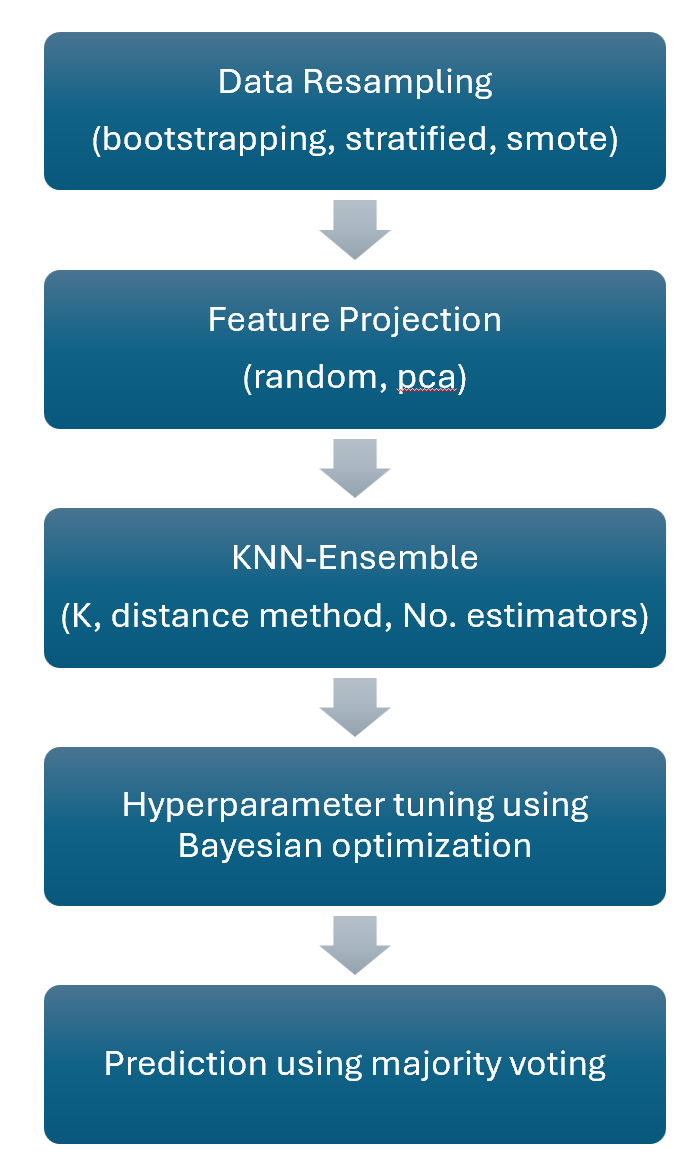
\includegraphics[width=0.2\linewidth]{OFU-xAI-Proj-Template_v0.2/images/PurposeMethod.png}
    \caption{Outline of our purpose method}
    \label{fig:purposeMethod}
\end{figure}


\subsubsection{Data Resampling}
We utilize various bootstrapping techniques to create multiple samples from the original dataset.

\textbf{Stratified Sampling}: Stratified sampling ensures that each subsample has the same proportion of classes as the original dataset. This is particularly useful for maintaining class distribution in imbalanced datasets \citep{stratified}. 


\textbf{SMOTE (Synthetic Minority Over-sampling Technique}:
SMOTE generates synthetic samples for the minority class by interpolating between existing minority class samples. This helps balance the dataset by increasing the number of minority class samples \citep{smote}.

\textbf{3- Bootstrapping}: Bootstrapping involves creating multiple samples from the original dataset by sampling with replacement. Each bootstrap sample is used to train a model, and the predictions are aggregated to improve accuracy and robustness.


\subsubsection{Feature Projection}
Our model uses two primary dimensionality reduction techniques to handle high-dimensional data efficiently: Random Gaussian Projection and Principal Component Analysis (PCA). These methods help to simplify the data while preserving its essential characteristics, improving both the performance and efficiency of our machine learning model.

\textbf{Random Gaussian Projection}: Random Gaussian Projection reduces the dimensionality of the data by projecting it onto a lower-dimensional subspace using a random matrix with Gaussian-distributed entries. This method is computationally efficient and preserves the distances between data points \cite{randomProjection}.
\begin{itemize}
    \item \textbf{Formula:} \( X' = X \cdot R \) \end{itemize}

where \( X \) is the original data matrix with dimensions \( N \times D \) (N samples and D features), \( R \) is a random matrix with dimensions \( D \times d \) (D original features and d reduced dimensions), and \( X' \) is the transformed data matrix with dimensions \( N \times D \). The entries of \( R \) are drawn from a Gaussian distribution with mean 0 and variance \( \frac{1}{d} \).

\textbf{Principal Component Analysis (PCA)}: PCA is a statistical technique that transforms the data into a new coordinate system such that the greatest variance by any projection of the data comes to lie on the first principal component, the second greatest variance on the second principal component, and so on. PCA captures the most significant features of the data, making it easier to analyze and visualize \citep{PCA}.

\begin{itemize}
    \item \textbf{Steps and Formulas:}
    \begin{enumerate}
        \item \textbf{Standardize the Data:} \( X_{\text{standardized}} = \frac{X - \mu}{\sigma} \) 
        
        where \( X \) is the original data matrix, \( \mu \) is the mean, and \( \sigma \) is the standard deviation.
        
        \item \textbf{Compute the Covariance Matrix:} \( \Sigma = \frac{1}{N-1} X_{\text{standardized}}^T X_{\text{standardized}} \) \\
        where \( \Sigma \) is the covariance matrix.
        
        \item \textbf{Compute the Eigenvalues and Eigenvectors:} Solve the eigenvalue equation:
        \[
        \Sigma v = \lambda v
        \]
        where \( \lambda \) are the eigenvalues and \( v \) are the eigenvectors.
        
        \item \textbf{Select Principal Components:} Choose the top \( d \) eigenvectors corresponding to the largest eigenvalues to form a matrix \( V \) with dimensions \( D \times d \).
        
        \item \textbf{Transform the Data:} \( X' = X_{\text{standardized}} \cdot V \) \\
        where \( X' \) is the transformed data matrix with dimensions \( N \times d \).
    \end{enumerate}
\end{itemize}


\subsubsection{KNN-Ensemble}
The KNN-Ensemble structure illustrated in Figure~\ref{fig:kNN-Ensemble} combines multiple KNN models to create a robust and accurate predictive model.

\begin{figure}[ht]
    \centering
    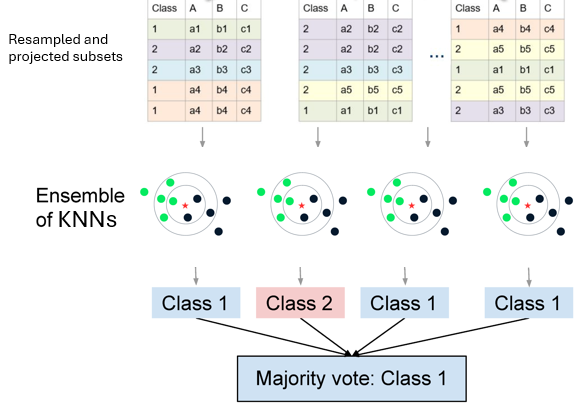
\includegraphics[width=0.6\linewidth]{OFU-xAI-Proj-Template_v0.2/images/kNN-Ensemble.png}
    \caption{KNN-Ensemble structure}
    \label{fig:kNN-Ensemble}
\end{figure}

KNN-Ensemble contains multiple KNN models, each represented by a circle. These models are trained on different resampled projected subsets of the training data. Each KNN model predicts a class label for the input. The final prediction is determined by majority voting. The class with the most votes among the individual KNN model predictions is selected as the final output.
Three key hyperparameters are tuned in the kNN-Ensemble structure to optimize performance. (1) number of estimators which refers to the number of kNN models in the ensemble. (2) K (Number of Neighbors). This parameter determines how many nearest neighbors each kNN model considers when making a prediction. (3) Distance Method. Different distance metrics can be used to calculate the distance between data points. The choice of distance metric can significantly affect the performance of the kNN models. The three common distance methods used are:

\begin{enumerate}
    \item \textbf{Cosine Distance:}
    \begin{itemize}
        \item Measures the cosine of the angle between two vectors. It is useful for comparing the orientation of the data points rather than their magnitude.
        \[
        \text{Cosine Distance} = 1 - \cos(\theta) = 1 - \frac{\vec{A} \cdot \vec{B}}{\|\vec{A}\| \|\vec{B}\|}
        \]
    \end{itemize}
    
    \item \textbf{Manhattan Distance:}
    \begin{itemize}
        \item Also known as L1 distance, it calculates the distance between two points by summing the absolute differences of their coordinates. It is useful for grid-like data structures.
        \[
        \text{Manhattan Distance} = \sum_{i=1}^{n} | A_i - B_i |
        \]
    \end{itemize}
    
    \item \textbf{Euclidean Distance:}
    \begin{itemize}
        \item Also known as L2 distance, it measures the straight-line distance between two points in space. It is the most common distance metric.
        \[
        \text{Euclidean Distance} = \sqrt{\sum_{i=1}^{n} (A_i - B_i)^2}
        \]
    \end{itemize}
    
\end{enumerate}


\subsubsection{Bayesian Optimization}

Bayesian Optimization is a powerful method for optimizing the hyperparameters of machine learning models. It is particularly effective for tuning models with expensive evaluation functions, where traditional grid search or random search methods may be inefficient. The main goal of Bayesian Optimization is to find the optimal set of hyperparameters that minimize or maximize the objective function, often the validation error of the model \citep{hyperparameter_Bayesian}.

\textbf{Key Concepts}

\begin{enumerate}
    \item \textbf{Surrogate Model:}
    \begin{itemize}
        \item Bayesian Optimization uses a probabilistic surrogate model to approximate the objective function. A common choice for the surrogate model is Gaussian Process (GP).
        \item \textbf{Formula:} The GP model predicts the mean ($\mu$) and variance ($\sigma^2$) of the objective function at a given point.
        \[
        f(x) \sim GP(\mu(x), \sigma^2(x))
        \]
    \end{itemize}
    
    \item \textbf{Acquisition Function:}
    \begin{itemize}
        \item The acquisition function determines the next point to evaluate by balancing exploration (uncertainty) and exploitation (expected improvement).
        \item Common acquisition functions include Expected Improvement (EI) and Upper Confidence Bound (UCB).
        \item \textbf{Formula for Expected Improvement (EI):}
        \[
        EI(x) = (\mu(x) - f(x^+))\Phi(Z) + \sigma(x)\phi(Z)
        \]
        Where $Z = \frac{\mu(x) - f(x^+)}{\sigma(x)}$, $\Phi$ is the cumulative distribution function, and $\phi$ is the probability density function of the standard normal distribution.
    \end{itemize}
    
\end{enumerate}



The Bayesian optimization algorithm is shown in Algorithm \ref{alg:bayesian_optimization}, where \( D_{1:t} = \{D_{1:t-1}, (x_t, y_t)\} \) represents the training dataset which consists of \( t-1 \) observations of the function \( f \). From the description of the algorithm, we can see that the whole algorithm is composed of two parts: Updating the posterior distribution (steps 3 and 4) and maximizing the acquisition function (step 2). As the observations accumulate, the posterior distribution is updated continuously; based on the new posterior, the point where the acquisition function is maximized is found and added to the training dataset. The whole process is repeated until the maximum number of iterations is reached or the difference between the current value and the optimal value obtained so far is less than a predefined threshold. It is noted that Bayesian optimization does not require the explicit expression of the function \( f \) \citep{practical_Bayesian}.


\begin{algorithm}
\caption{Bayesian optimization}
\label{alg:bayesian_optimization}
\begin{algorithmic}[1]
\For{$t = 1, 2, \dots$}
    \State Find $x_t$ by optimizing the acquisition function $u$ over function $f$:
    \[
    x_t = \arg\max_x u(x|D_{1:t-1}).
    \]
    \State Sample the objective function: $y_t = f(x_t)$.
    \State Augment the data $D_{1:t} = \{D_{1:t-1}, (x_t, y_t)\}$ and update the posterior of function $f$.
\EndFor
\end{algorithmic}
\end{algorithm}

\subsubsection{Majority voting}
After training and finding the best configuration of the Forest-KNN model, we use majority voting to determine the final prediction. Each KNN model in the ensemble makes its prediction, and the class with the most votes across these predictions is selected as the final output. This method ensures that the final decision leverages the strengths of all individual models, enhancing robustness and accuracy.



\subsection{Model Architectures}
\subsubsection{Simple kNN}\label{simpleknn}
To evaluate the performance of the k-Nearest Neighbour (kNN) classifier for Step 1, we implemented a custom kNN model using PyTorch, enabling the use of GPU acceleration. The kNN algorithm classifies a data point by identifying the k closest points in the training set and assigning the majority class among these neighbors. The kNN classifier is initialized with the number of neighbors k and the device (CPU or GPU) on which computations are performed. The training process involves storing the training data and corresponding labels as PyTorch tensors on the specified device. During prediction, the classifier computes pairwise distances between the input data and the training data using the Euclidean distance metric. The nearest neighbors are identified by sorting these distances. The class labels of the nearest neighbors are then used to predict the class of each input sample by taking the mode (most common label) of these labels.

\subsubsection{Simple Linear Layer}\label{simplelinearlayer}
The Linear Probing method involves training a simple linear classifier using the feature representations (embeddings) from the datasets. This method aims to improve classification by using a single layer neural network directly on the embeddings. The Linear Layer is initialized with the input dimension, representing the feature size of the embeddings, and the number of classes in the dataset. The training process involves defining a loss function (Cross-Entropy Loss) and an optimizer (Adam). The model is trained by performing forward and backward passes to minimize the loss function over a series of epochs. The training data is fed into the linear layer, and the model parameters are updated to improve classification accuracy. Hyperparameter tuning is performed by training the model with various learning rates, batch sizes, and epochs. The performance on the validation set is monitored to identify the best set of hyperparameters.

\subsubsection{ForestKNN}
To assess the capabilities of the Forest k-Nearest Neighbors (Forest-KNN) model, we developed an ensemble of custom KNN classifiers with PyTorch, utilizing GPU acceleration for faster processing. The Forest-KNN model aggregates the predictions from multiple KNN classifiers, each trained on distinct subsets of the dataset. This implementation involves storing the training data and labels as PyTorch tensors on the GPU. During inference, the model calculates the distances between each input data point and the stored training points using the chosen distance metric, such as Euclidean. Each KNN classifier identifies its k nearest neighbors from its specific training subset and predicts the input data's class based on the majority class among these neighbors. The ensemble's final prediction for each sample is determined by combining the individual predictions from all classifiers, usually through a majority voting mechanism. This ensemble method enhances prediction reliability and accuracy by leveraging diverse training subsets.

\section{Experiments}\label{experiments}
\subsection{Datasets}\label{datasets}
Our experimental framework focuses on the use of four central datasets: CIFAR-10, CIFAR-100, DermaMNIST, and BreastMNIST, each of which is briefly introduced here.

\subsubsection{CIFAR-10}\label{cifar10}
The CIFAR-10 dataset consists of 60,000 32×32 color images in 10 different classes, with 6,000 images per class, ensuring a balanced dataset. These classes include airplanes, cars, birds, cats, deer, dogs, frogs, horses, ships, and trucks \citep{Krizhevsky2009}. The dataset is split into a training set of 50,000 images and a test set of 10,000 images. Each image is labeled with one of the 10 classes, providing a robust benchmark for evaluating image recognition algorithms. The embeddings provided for this dataset have 768 dimensions. Some examples of the CIFAR-10 dataset can be seen in Figure~\ref{fig:combined}.

\subsubsection{CIFAR-100}\label{cifar100}
Similar to CIFAR-10, the CIFAR-100 dataset contains 60,000 32×32 color images, balanced across 100 classes, with 600 images per class. The classes are grouped into 20 superclasses, with each image labeled at two levels of granularity: a coarse label (superclass) and a fine label (class) \citep{Krizhevsky2009}. The dataset is also divided into a training set of 50,000 images and a test set of 10,000 images. CIFAR-100 is more challenging than CIFAR-10 due to its larger number of classes and the finer granularity of the labels. The embeddings provided for this dataset have 768 dimensions. Some examples are also given in Figure~\ref{fig:combined}.

\subsubsection{DermaMNIST}\label{dermamnist}
The DermaMNIST subset of the MedMNIST collection focuses on dermatological image classification, specifically for skin lesion analysis. The dataset includes 10,015 ''multi-source dermatoscopic images of common pigmented skin lesions'' \citep{medmnistv1, medmnistv2}. The images are classified into seven categories: actinic keratoses, basal cell carcinoma, benign keratosis-like lesions, dermatofibroma, melanocytic nevi, melanoma, and vascular lesions \citep{DBW86T_2018}. Originally, the images were high resolution (3 × 600 × 450), but for this project, they were resized to 3 × 28 × 28 pixels. The dataset is split into a training set of 7,007 samples, a validation set of 1003 samples, and a test set of 2,005 samples. The embeddings provided for this project for this dataset have 768 dimensions. Some examples are shown in Figure~\ref{fig:combined}.


\subsubsection{BreastMNIST}\label{breastmnist}
The BreastMNIST subset is another component of the MedMNIST collection, designed for breast ultrasound image classification. It contains 780 images categorized into three classes: normal, benign, and malignant. For this project, the task was simplified to binary classification ''by combining normal and benign as positive and classifying them against malignant as negative'' \citep{medmnistv1, medmnistv2}. The original high-resolution images (500 × 500) were resized to 28 × 28 pixels. The dataset is divided into a training set of 546 samples, a validation set of 78 samples, and a test set of 156 samples. The given embeddings also were of size 768. Some examples of the BreastMNIST dataset can be seen in Figure~\ref{fig:combined}.


\begin{figure}[ht]
  \centering
  \begin{minipage}{0.61\linewidth}
    \parbox[b]{0.2\linewidth}{
      \raggedleft \scriptsize CIFAR-10
    }
    \adjustbox{valign=m}{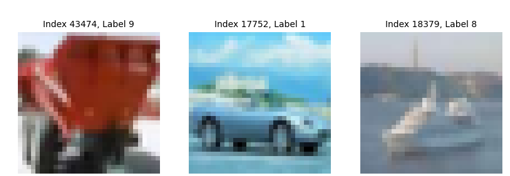
\includegraphics[width=0.7\linewidth]{images/cifar10_images.png}}
  \end{minipage}

  \begin{minipage}{0.615\linewidth}
    \parbox[b]{0.2\linewidth}{
      \raggedleft \scriptsize CIFAR-100
    }
    \adjustbox{valign=m}{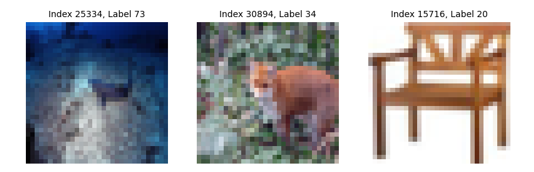
\includegraphics[width=0.7\linewidth]{images/cifar100_images.png}}
  \end{minipage}
  
  \begin{minipage}{0.6\linewidth}
    \parbox[b]{0.2\linewidth}{
      \raggedleft \scriptsize DermaMNIST
    }
    \adjustbox{valign=m}{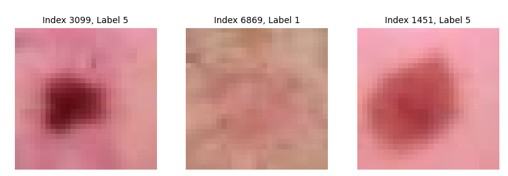
\includegraphics[width=0.7\linewidth]{images/dermamnist_images.png}}
  \end{minipage}
  
  \begin{minipage}{0.615\linewidth}
    \parbox[b]{0.2\linewidth}{
      \raggedleft \scriptsize BreastMNIST
    }
    \adjustbox{valign=m}{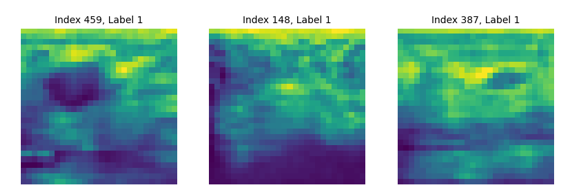
\includegraphics[width=0.7\linewidth]{images/breastmnist_images.png}}
  \end{minipage}

  \caption{Example images of the datasets: CIFAR-10, CIFAR-100, DermaMNIST, and BreastMNIST.}
  \label{fig:combined}
\end{figure}


\subsection{Data Preparation}
For loading the data, we used the given embeddings and labels from the CIFAR-10, CIFAR-100, DermaMNIST, and BreastMNIST datasets, stored in numpy files. The indices of the vector databases matched those of the original image databases, allowing us to map the embeddings to the original images for representation purposes. For datasets without predefined validation sets, the training data was split into training and validation sets (80/20 split) to facilitate model evaluation and hyperparameter tuning. The data was normalized to ensure consistent feature scaling, which is important for the performance of distance-based algorithms like kNN\@.


\subsection{Step 1 - Analyze Data}
The first step of this project involved analyzing and understanding the given embedding space of the data. We began by visualizing the latent spaces using t-distributed Stochastic Neighbor Embedding (t-SNE) plotting \citep{Maaten2008}, which reduced the high-dimensional data (768 dimensions) to two dimensions. This reduction revealed patterns and class overlaps, allowing us to create a colored 2D plot that showed clusters for each label within the data.

Simply having an overview was not sufficient to gain deeper insights, so we examined randomly selected indices and analyzed their nearest neighbors. This approach enabled us to identify connections and similarities among neighboring points. However, the random selection often resulted in similar images for the same label, lacking diversity.

To enhance our evaluation, we specifically focused on points in the dataset that had several nearest neighbors with different labels. For example, as shown in Figure \ref{fig:cifar10_combined}, we selected a point with index 151 from the CIFAR-10 dataset and identified its five nearest neighbors. This method allowed us to identify edge cases where points were positioned between several classes, helping us understand why an image was labeled as it was.

Additionally, we marked the selected index within the t-SNE plot, as well as its nearest and furthest points. Although the t-SNE plot might not visually represent the nearest or furthest points accurately due to dimensionality reduction, these points are indeed the true neighbors or furthest points in the original high-dimensional space. This approach, illustrated in Figure \ref{fig:cifar10_combined} for the CIFAR-10 dataset, has helped us to understand the internals of the embedding space a little better. Similar t-SNE plots and selected indices with neighbors for the other datasets can be found in the appendix: Figure \ref{fig:cifar100_combined}, Figure \ref{fig:dermamnist_combined}, Figure \ref{fig:breast_combined}.

\begin{figure} [ht]
    \centering
    \begin{minipage}{1\linewidth}
        \centering
        \adjustbox{scale=1.3,center}{
            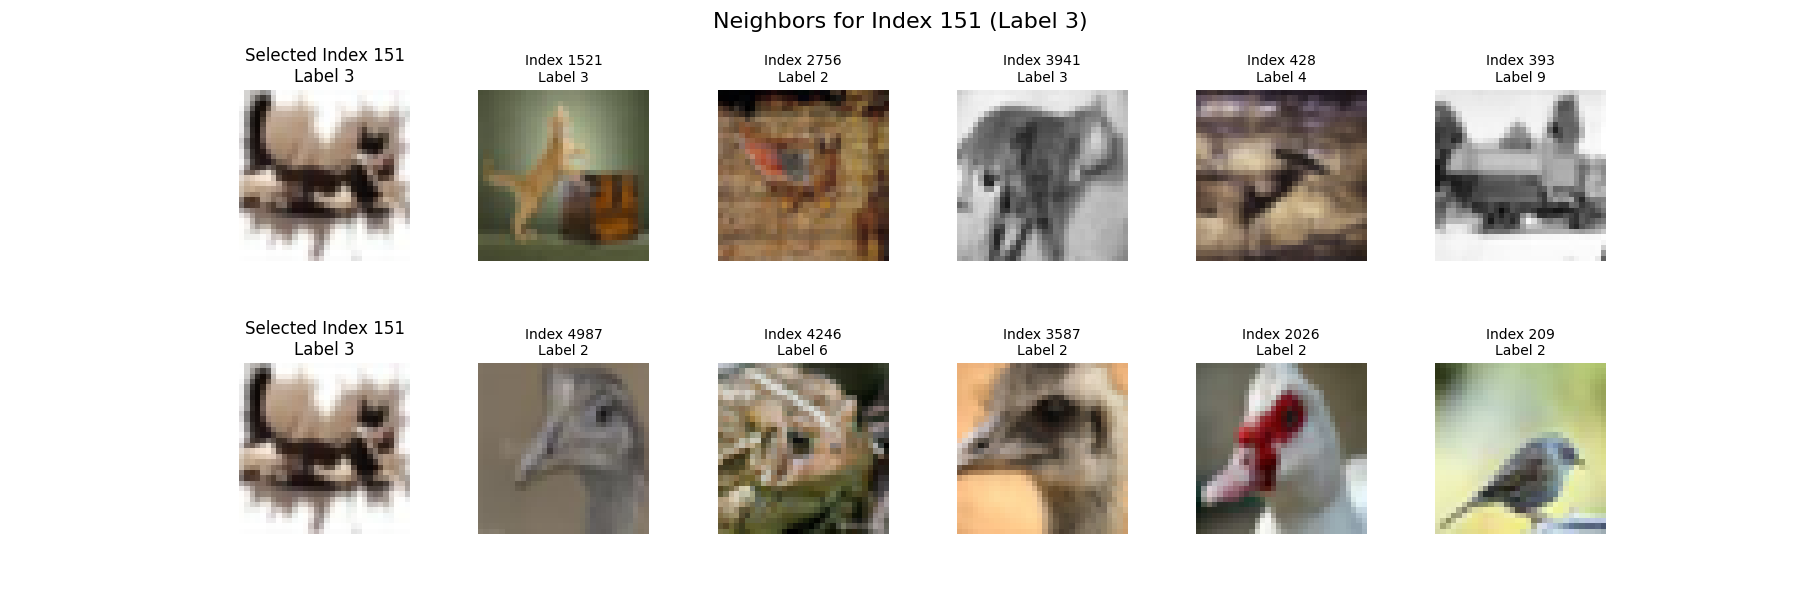
\includegraphics[width=\linewidth]{OFU-xAI-Proj-Template_v0.2/images/cifar10_index151_subsampled_neighbors.png}
        }
    \end{minipage}\hfill
    \begin{minipage}{1\linewidth}
        \centering
        \adjustbox{scale=.9,center}{
            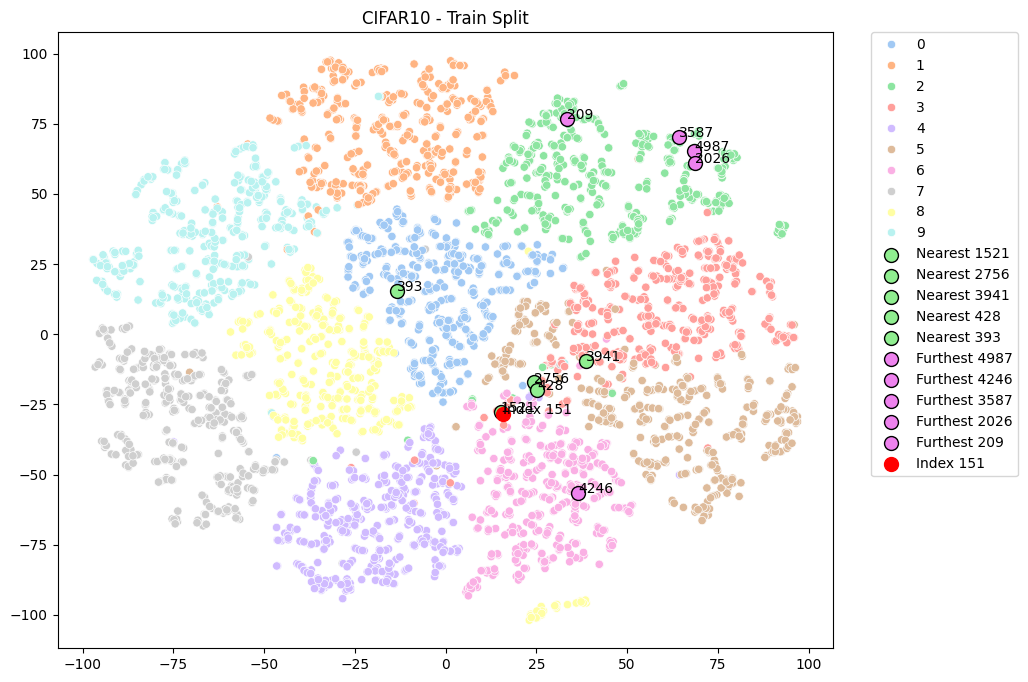
\includegraphics[width=\linewidth]{OFU-xAI-Proj-Template_v0.2/images/cifar10_index151_subsampled_tsne.png}
        }
    \end{minipage}
    \caption{Top: Nearest neighbors for the point with index 151 in CIFAR-10 dataset, illustrating class overlap. Bottom: t-SNE plot of CIFAR-10 dataset showing clusters of different labels in a 2D space.}
    \label{fig:cifar10_combined}
\end{figure}

\subsection{Step 2 - Compare SimpleKNN with Linar Layer}
As working with kNNs is a novel task for us, our initial idea was to briefly introduce ourselves to this domain and use a simple approach to work with the given vector databases. For this, we created a simple kNN class as outlined in Section~\ref{simpleknn}. Our goal was to evaluate different values of k (1, 3, 5, 7, 9, 11, 13, 15, 20, 30, 40) and assess the effectiveness of these values. For comparison, we also implemented a simple, one-layered linear model, which is described in Section~\ref{simplelinearlayer}. For this model, we evaluated several hyperparameters.

We started with the kNN model, training it on the training set and evaluating its performance on the validation set for each value of k. The validation accuracy was calculated for each k, and the optimal k value was determined based on the highest validation accuracy. The best k value was then used to evaluate the model on the test set. We recorded performance metrics such as accuracy, precision, recall, and F1 score to comprehensively assess the classifier's effectiveness. Additionally, we recorded the indices of misclassified samples but were unable to determine the reasons behind these misclassifications, as the internal learning process of the models does not provide clear insights into their decision-making.

In parallel, we trained the linear layer model. We performed hyperparameter tuning by conducting a grid search over the specified learning rates (0.001, 0.005), batch sizes (32, 64), and number of epochs (20, 40). The model was trained on the training set and validated on the validation set for each combination of hyperparameters. The best set of hyperparameters was selected based on the highest validation accuracy. The final model, trained with the best hyperparameters, was then evaluated on the test set, and performance metrics were recorded similarly to the kNN model.

A detailed comparison of the performance metrics for both methods across all datasets can be found in the Appendix (Table \ref{tab:step2_results}).


\subsection{Step 3 - ForestKNN}
The problem of implementing a ForestKNN for step 3 was a major challenge as we had to significantly improve our simple kNN approach. To understand the impact of each component described above, we gradually improved our original kNN model by adding functionality incrementally. This systematic approach allowed us to evaluate the contribution of each component to overall performance.
First, we added bootstrapping to our kNN model. Bootstrapping involved creating multiple subsets of the training data through random sampling with replacement. Each subset was used to train a separate kNN classifier. This improvement was intended to improve the robustness of the model by reducing the variance.
As the BreastMNIST and DermamNIST datasets were unbalanced, we also attempted to equalize the data using the Synthetic Minority Over-sampling Technique (SMOTE). However, this approach resulted in significantly lower accuracy, so we discarded it. 
Next, we explored various distance metrics to determine which would perform best for our kNN models. We experimented with a comprehensive set of metrics, including Euclidean, Cosine, Manhattan, Chebyshev \citep{chebyshev1867}, Minkowski \citep{minkowski1896}, Mahalanobis \citep{mahalanobis1936}, and Canberra \citep{lance1967} distances. Each metric was evaluated, and we selected the most effective metrics for our final ForestKNN approach.
In addition, we experimented with using different k-values for different subtrees within the ensemble. The evaluated k-values included groups such as [1, 3, 5], [3, 5, 7] and [5, 7, 9]. This approach allowed us to include diversity within the ensemble by using different k-values for different classifiers.
The final step in our enhancement process involved combining all approaches using Bayesian optimization

Detailed results of the intermediate steps and the final model's performance are provided in Appendix Table \ref{tab:v_accuracy_incremental}. It is worth noting that we only evaluated the results of the stepwise approach for the BreastMNIST dataset, as the overall complexity of the ForestKNN increased with additional features. Given our limited computational power locally, we were unable to compute the results for the other, larger datasets such as CIFAR-10, CIFAR-100, and DermamNIST. Especially when trying various distances, we quickly reached the limit and encountered GPU memory errors. We have therefore decided to limit ourselves to a smaller selection.



\subsubsection{Tuning Hyperparameters}
Table\ref{tab:hyperparameters} outlines the key hyperparameters and their respective search spaces that are tuned in our Ensemble KNN model using Bayesian Optimization. These hyperparameters include the resampling method (SMOTE, Stratified Sampling, Bootstrapping), the projection method (Random Gaussian Projection, PCA), the number of components in random projection (50, 100, 150), the variance threshold in PCA (0.90, 0.99), the number of estimators (10, 30), the number of nearest neighbors (K) (3, 10), and the distance metric (Cosine, Euclidean, Manhattan). This comprehensive tuning process aims to optimize the model's performance by exploring a wide range of parameter values.

\begin{table}[ht]
    \caption{Hyperparameters tuning search space}
    \label{tab:hyperparameters}
    \centering
    \begin{tabular}{>{\raggedright}m{0.4\linewidth} >{\raggedright\arraybackslash}m{0.5\linewidth}}
    \hline\hline
    \textbf{Hyperparameter} & \textbf{Search space} \\
    \hline
    Resampling method & [SMOTE, Stratified, Bootstrapping] \\
    \hline
    Projection method & [Random Gaussian Projection, PCA] \\
    \hline
    Number of components of random projection & [50, 100, 150] \\
    \hline
    Variance threshold in PCA & (0.90, 0.99) \\
    \hline
    Number of estimators & (10, 30) \\
    \hline
    K (number of nearest neighbors) & (3, 10) \\
    \hline
    Distance metric & [Cosine, Euclidean, Manhattan] \\
    \hline
    \end{tabular}
\end{table}




\section{Discussion}
\subsection{Step 2}
The results from Step 2 highlight several insights into the performance of simple k-Nearest Neighbor (kNN) and Linear Probing methods across various datasets. Overall, Linear Probing generally outperformed kNN, particularly in more complex datasets.

For CIFAR-10, both methods performed well, with kNN achieving a slightly higher validation accuracy of 98.70\% compared to 98.62\% for Linear Probing. In the more complex CIFAR-100 dataset, Linear Probing was superior, achieving 90.48\% validation accuracy versus kNN’s 89.50\%. DermaMNIST results were close, with kNN slightly ahead at 79.35\% validation accuracy compared to Linear Probing’s 78.60\%. For BreastMNIST, Linear Probing significantly outperformed kNN, with a validation accuracy of 85.26\% compared to 79.49\%.

These results suggest that both methods are suitable for datasets with distinct class boundaries, while Linear Probing is better at handling datasets with higher class diversity, likely due to its ability to learn feature weights. Despite kNN's slight edge in some cases, the higher validation accuracy of Linear Probing indicates better generalization to unseen data, highlighting its potential for medical image classification.

Overall, the findings suggest that while the simple kNN method provided reasonable results, it was not optimized for high performance. Linear Probing, despite using only a single linear layer, showed promising results that could be significantly improved with more advanced architectures and hyperparameter optimization. The detailed comparison of performance metrics in the Appendix supports these conclusions and suggests directions for future enhancements.



\subsection{Step3}

\begin{table}[ht]
    \caption{Forest-KNN results across datasets}
    \label{tab:comparison_HP}
    \centering
    \begin{tabular}{>{\raggedright}m{0.25\linewidth} >{\raggedright\arraybackslash}m{0.15\linewidth} >{\raggedright\arraybackslash}m{0.15\linewidth} >{\raggedright\arraybackslash}m{0.15\linewidth} >{\raggedright\arraybackslash}m{0.15\linewidth}}
    \hline
    \textbf{} & \textbf{Cifar 10} & \textbf{Cifar100} & \textbf{DermaMNIST} & \textbf{BreastMNIST} \\
    \hline
    Resampling method & Bootstrapping & Stratified & Stratified & Bootstrapping \\
    \hline
    Projection method & Random G & Random G & Random G & Random G \\
    \hline
    Number of components of random projection & 139 & 100 & 72 & 94 \\
    \hline
    Variance threshold in PCA & - & - & - & - \\
    \hline
    Number of estimators & 28 & 20 & 16 & 26 \\
    \hline
    K (number of nearest neighbors) & 9 & 5 & 3 & 3 \\
    \hline
    Distance metric & Euclidean & Euclidean & Euclidean & Euclidean \\
    \hline
    Accuracy & 0.9873 & 0.899 & 0.880 & 0.871 \\
    \hline
    \end{tabular}
\end{table}


Table \ref{tab:comparison_HP} shows the selected best hyperparameters and the accuracy of our purpose model Forest-KNN across various datasets. For the CIFAR-10 dataset, using bootstrapping and random Gaussian projection with 139 components, 28 estimators, and 9 nearest neighbors, the model achieved an impressive accuracy of 98.73\%. Similarly, for CIFAR-100 and BreastMNIST, stratified sampling and random Gaussian projection yielded accuracies of 89.9\% and 87.1\%, respectively, with optimal settings. For DermaMNIST, stratified sampling with 72 components, 16 estimators, and 3 nearest neighbors led to an accuracy of 88.0\%. All datasets consistently performed best with the Euclidean distance metric.\\
Furthermore, we conducted a Feature importance analysis to determine the impact of each hyperparameter on model accuracy. Figure \ref{fig:HP_impact} depicts the importance of various hyperparameters on model accuracy for the BreastMNIST, DermaMNIST, CIFAR-10, and CIFAR-100 datasets. For BreastMNIST and DermaMNIST, the sampling method is the most influential hyperparameter, followed by the number of nearest neighbors (K), indicating the significant impact of resampling techniques and local data structures on these medical imaging datasets. The number of components in the random projection also plays a notable role. In contrast, for CIFAR-10 and CIFAR-100, the number of components and the number of estimators are the most important hyperparameters, highlighting the critical role of dimensionality reduction and ensemble size in these image classification tasks. Other hyperparameters, such as the distance method, variance threshold, and projection method, have minimal impact across all datasets. These insights emphasize the need for careful tuning of specific hyperparameters to optimize model performance for different types of data.

\begin{figure}
    \centering
    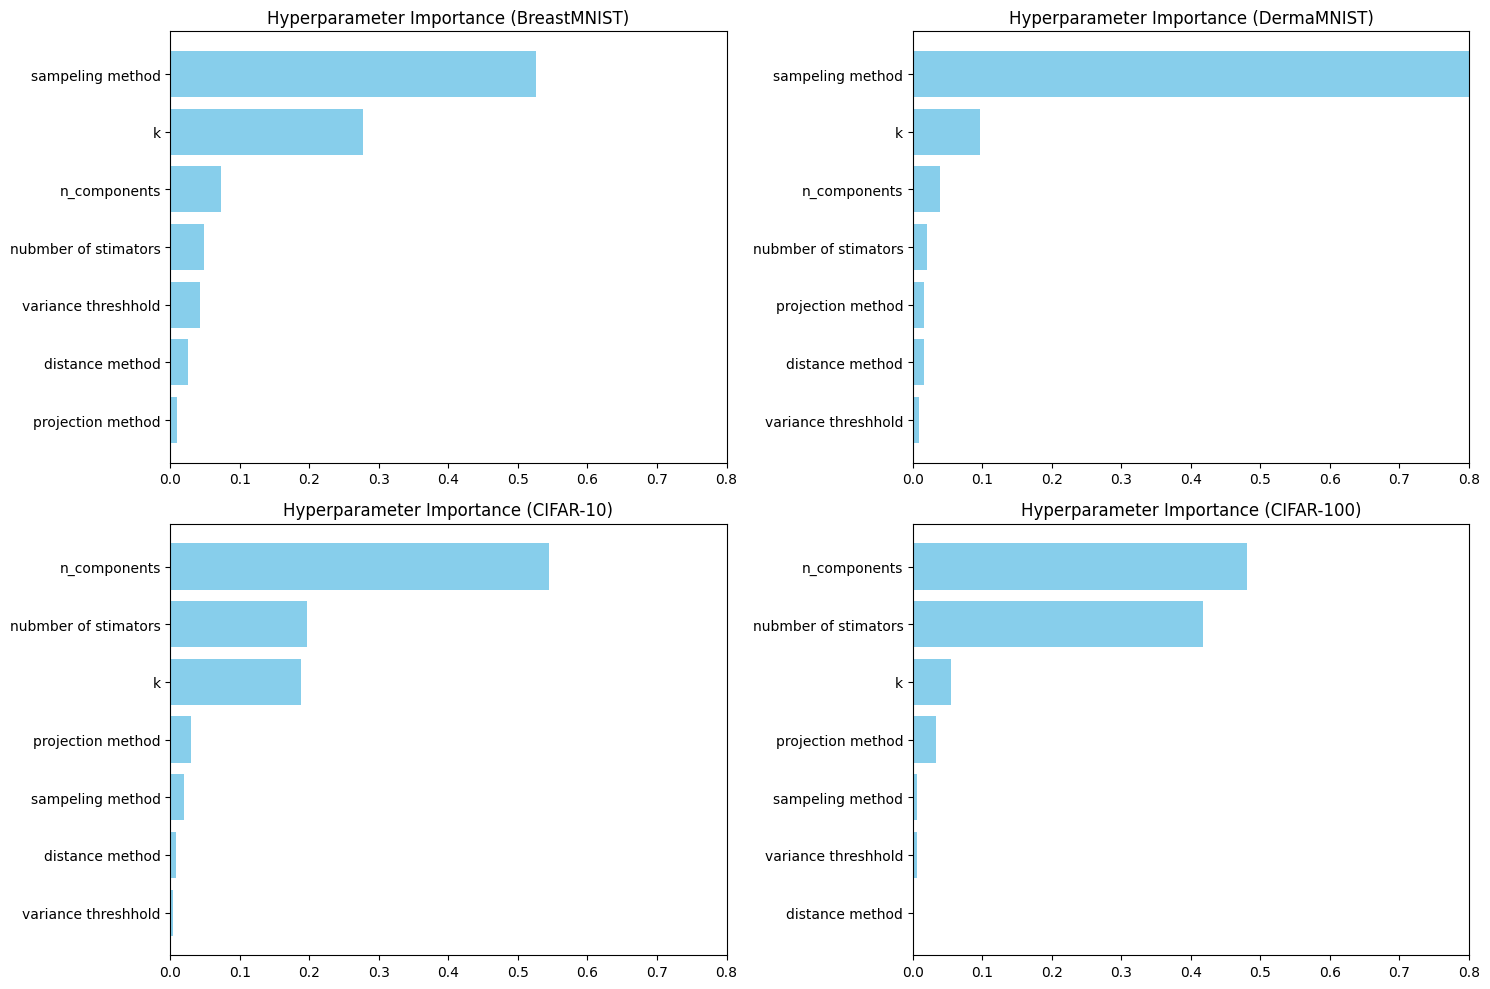
\includegraphics[width=0.99\linewidth]{OFU-xAI-Proj-Template_v0.2/images/HP_impact.png}
    \caption{Forest-KNN Hyperparameters feature importance o}
    \label{fig:HP_impact}
\end{figure}


\section{Conclusion}
In this project, we developed and refined the Forest-KNN model by combining k-Nearest Neighbor (kNN) algorithms with principles from Random Forests for image classification tasks. Our approach was applied to various datasets, including CIFAR-10, CIFAR-100, DermaMNIST, and BreastMNIST. We focused on enhancing the robustness and accuracy of the kNN model by employing resampling methods to create multiple training subsets and exploring different distance metrics such as Manhattan, Euclidean, and Cosine. Bayesian optimization was used to fine-tune the model parameters, achieving optimal performance. Our results indicated that Forest-KNN is a robust and efficient alternative to traditional kNN and linear models, capable of handling complex datasets effectively. However, the added functionality comes with an increased computational cost. While there were slight improvements across various datasets compared to simpler approaches, they were not always the highest. Nonetheless, the Forest-KNN model demonstrated improvements in classification accuracy and robustness, particularly in medical image classification, where precision is crucial. Future work could involve further optimization, scaling to larger datasets, and exploring additional ensemble strategies and distance metrics. This project highlights the potential of ensemble methods to enhance classification accuracy and robustness, providing valuable insights into the practical application of machine learning in complex datasets.

\bibliography{bibliography}
\bibliographystyle{abbrvnat}



\newpage
{\parindent 0cm}
%%%%%%%%%%%%%%%%%%%%%%%%%%German%%%%%%%%%%%%%%%%%%%%%%%%%%%%%%
\section*{Declaration of Authorship}
Ich erkläre hiermit gemäß § 9 Abs. 12 APO, dass ich die vorstehende Projektarbeit selbstständig verfasst und keine anderen als die angegebenen Quellen und Hilfsmittel benutzt habe. Des Weiteren erkläre ich, dass die digitale Fassung der gedruckten Ausfertigung der Projektarbeit ausnahmslos in Inhalt und Wortlaut entspricht und zur Kenntnis genommen wurde, dass diese digitale Fassung einer durch Software unterstützten, anonymisierten Prüfung auf Plagiate unterzogen werden kann.\\
\vspace{2\baselineskip}
  
Bamberg, \today

\rule[0.5em]{14em}{0.5pt} \hspace{0.25\linewidth}\rule[0.5em]{14em}{0.5pt}
\vspace{1em}
\hspace{4em} (Place, Date) \hspace{0.51\linewidth} (Signature)

Bamberg, \today

\rule[0.5em]{14em}{0.5pt} \hspace{0.25\linewidth}\rule[0.5em]{14em}{0.5pt}
\vspace{1em}
\hspace{4em} (Place, Date) \hspace{0.51\linewidth} (Signature)



%%%%%%%%%%%%%%%%%%%%%%%%%%%%%%%%%%%%%%%%%%%%%%%%%%%%%%%%%%%%


%%%%%%%%%%%%%%%%%%%%%%%%%%%%%%%%%%%%%%%%%%%%%%%%%%%%%%%%%%%%

\newpage
\appendix


\section{Appendix}

\begin{figure}[ht]
    \centering
    \begin{minipage}{1\linewidth}
        \centering
        \adjustbox{scale=1.3,center}{
            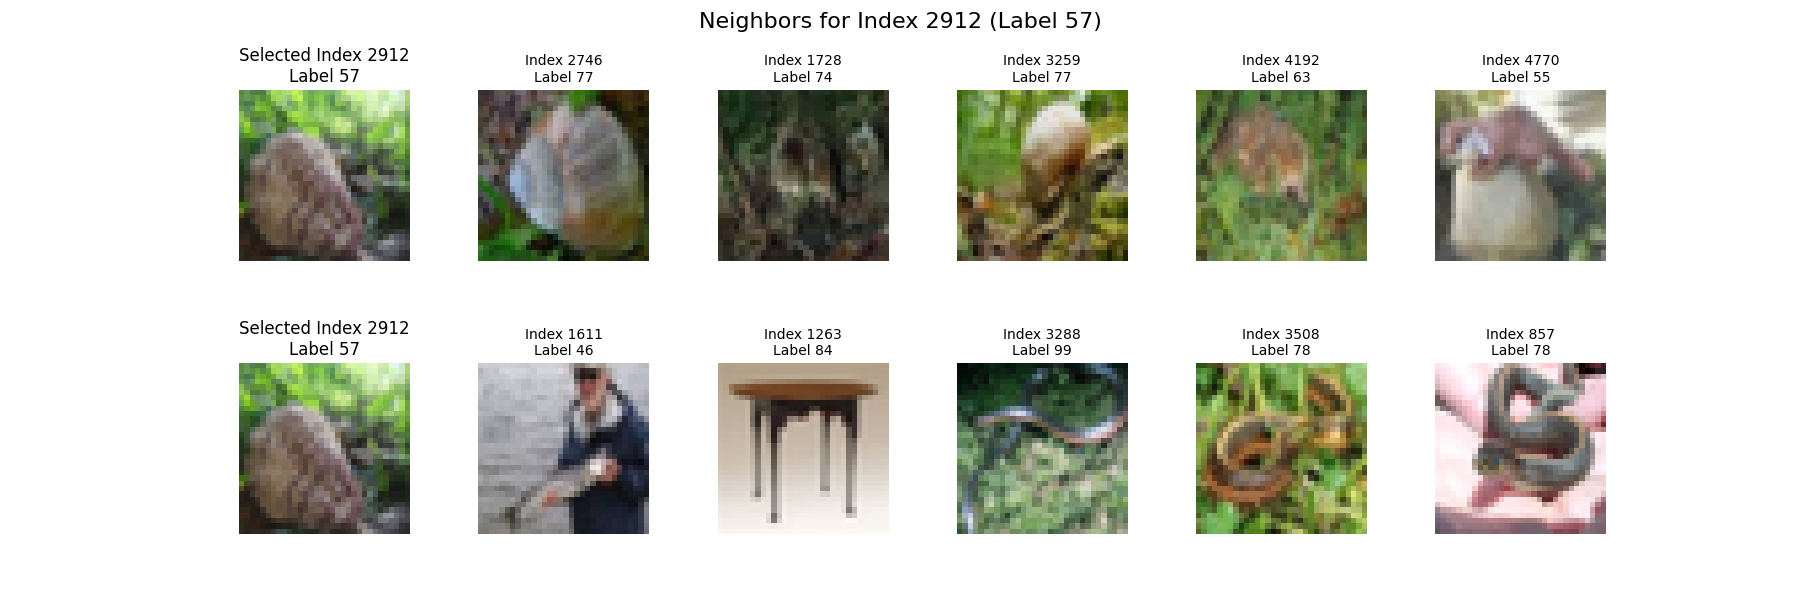
\includegraphics[width=\linewidth]{OFU-xAI-Proj-Template_v0.2/images/cifar100_index2912_subsampled_neighbors.png}
        }
    \end{minipage}\hfill
    \begin{minipage}{1\linewidth}
        \centering
        \adjustbox{scale=.9,center}{
            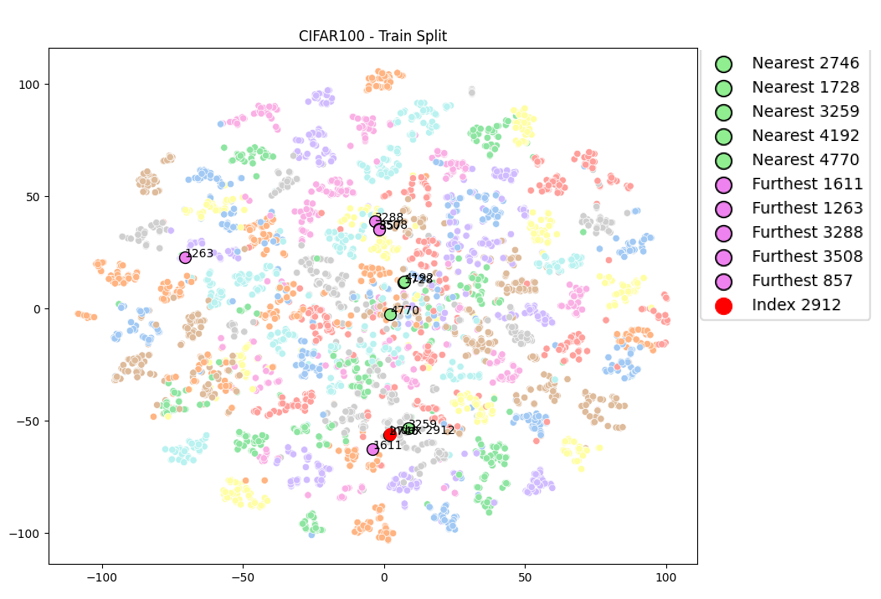
\includegraphics[width=\linewidth]{OFU-xAI-Proj-Template_v0.2/images/cifar100_index2912.png}
        }
    \end{minipage}
    \caption{Nearest neighbors and t-SNE for index 2912 in the CIFAR-100 dataset.}
    \label{fig:cifar100_combined}
\end{figure}

\begin{figure}[ht]
    \centering
    \begin{minipage}{1\linewidth}
        \centering
        \adjustbox{scale=1.3,center}{
            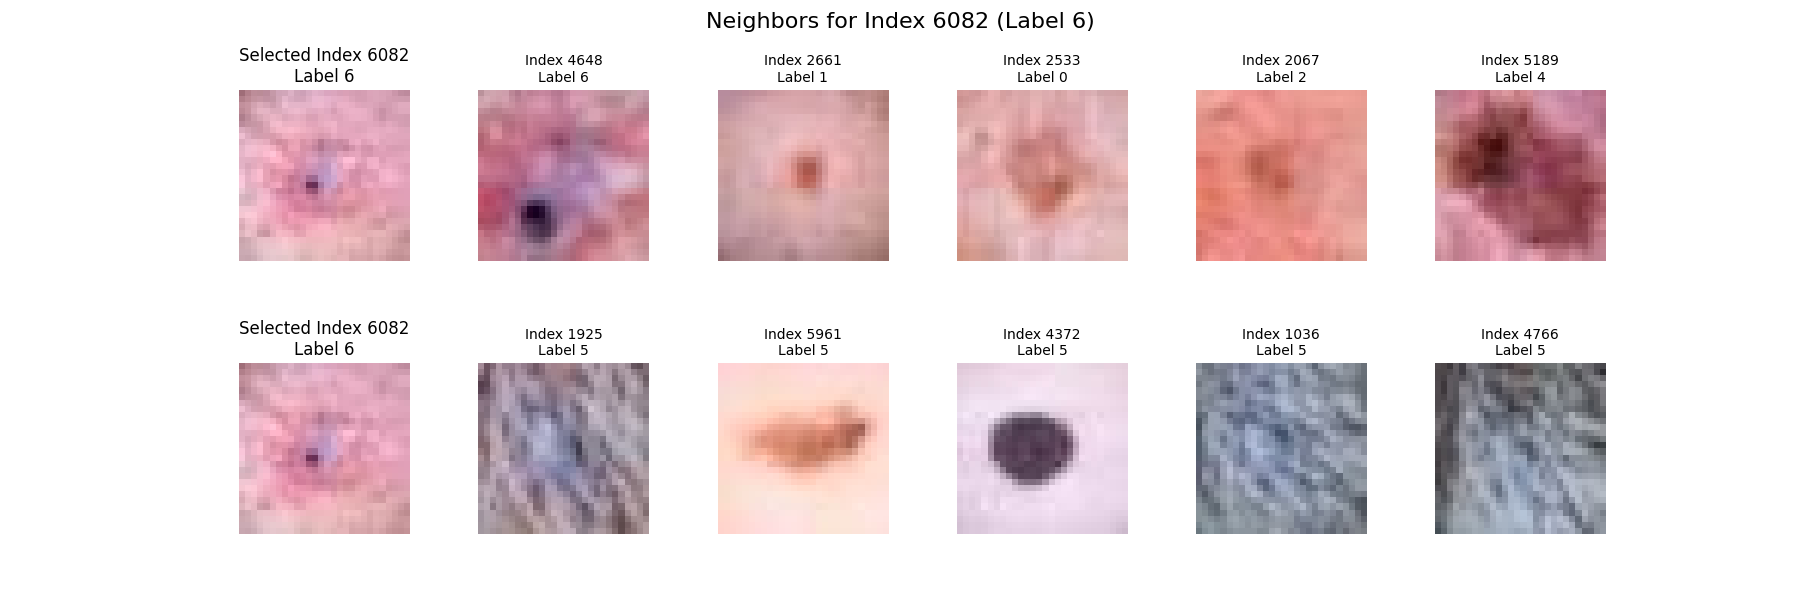
\includegraphics[width=\linewidth]{OFU-xAI-Proj-Template_v0.2/images/dermamnist_index6082_full_neighbors.png}
        }
    \end{minipage}\hfill
    \begin{minipage}{1\linewidth}
        \centering
        \adjustbox{scale=.9,center}{
            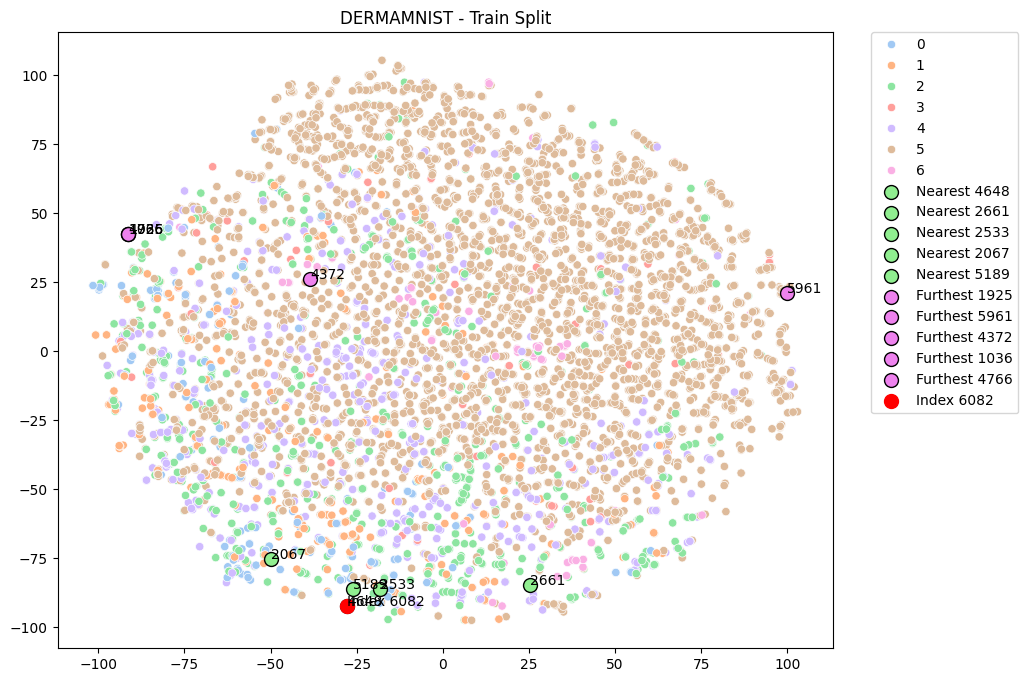
\includegraphics[width=\linewidth]{OFU-xAI-Proj-Template_v0.2/images/dermamnist_index6082_full_tsne.png}
        }
    \end{minipage}
    \caption{Nearest neighbors and t-SNE for index 6082 in DermaMNIST dataset}
    \label{fig:dermamnist_combined}
\end{figure}

\begin{figure}[ht]
    \centering
    \begin{minipage}{1\linewidth}
        \centering
        \adjustbox{scale=1.3,center}{
            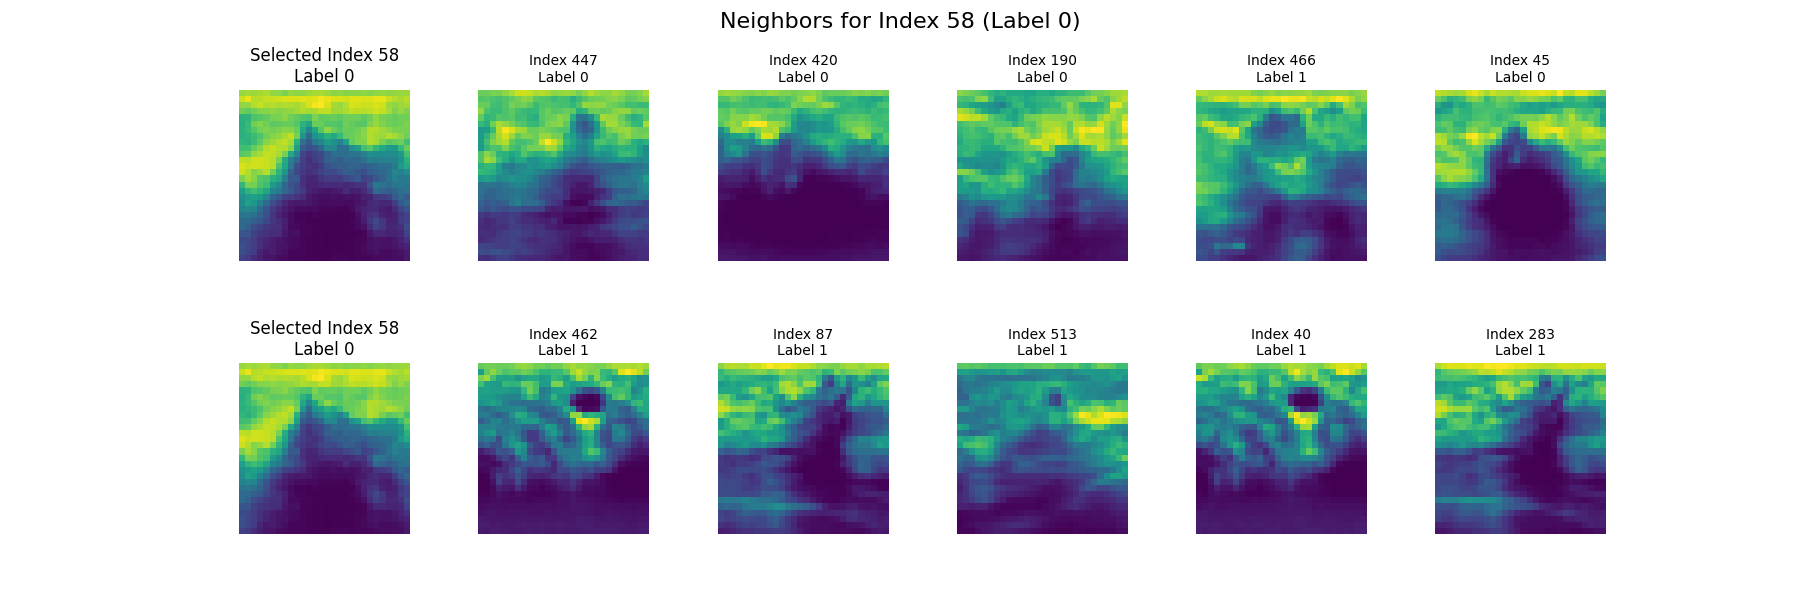
\includegraphics[width=\linewidth]{OFU-xAI-Proj-Template_v0.2/images/breastmnist_index58_full_neighbors.png}
        }
    \end{minipage}\hfill
    \begin{minipage}{1\linewidth}
        \centering
        \adjustbox{scale=.9,center}{
            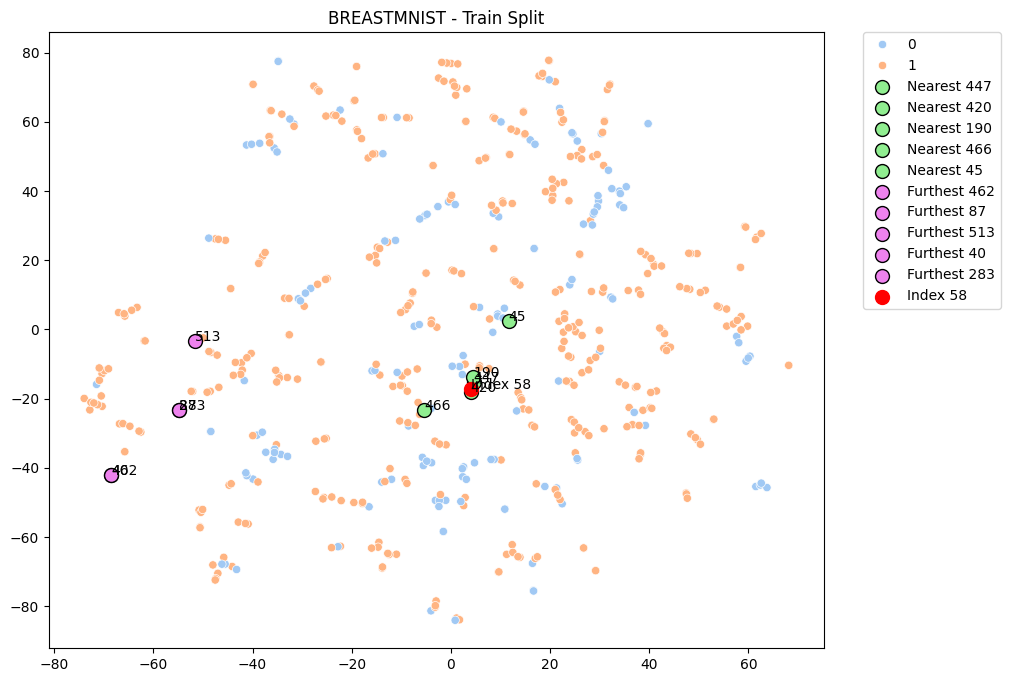
\includegraphics[width=\linewidth]{OFU-xAI-Proj-Template_v0.2/images/breastmnist_index58_full_tsne.png}
        }
    \end{minipage}
    \caption{Nearest neighbors and t-SNE for index 58 in BreastMNIST dataset.}
    \label{fig:breast_combined}
\end{figure}


\begin{table}[ht]
  \caption{Performance Comparison of Simple kNN and Linear Layer Methods for Step 2}
  \label{tab:step2_results}
  \centering
  \begin{tabular}{lll}
    \toprule
    \multicolumn{3}{c}{CIFAR-10} \\
    \cmidrule(r){1-3}
    Method & kNN & Linear Layer \\
    \cmidrule(r){1-3}
    Best Parameter(s) & \( k = 11 \) & lr=0.005, batch\_size=32, epochs=40 \\
    Validation Accuracy (\%) & \textbf{98.90} & 98.84 \\
    Test Accuracy (\%) & \textbf{98.70} & 98.62 \\
    Test Precision (\%) & \textbf{98.71} & 98.62 \\
    Test F1 Score (\%) & \textbf{98.70} & 98.62 \\
    \midrule
    
    \multicolumn{3}{c}{CIFAR-100} \\
    \cmidrule(r){1-3}
    Method & kNN & Linear Layer \\
    \cmidrule(r){1-3}
    Best Parameter(s) & \( k = 15 \) & lr=0.005, batch\_size=32, epochs=40 \\
    Validation Accuracy (\%) & 89.93 & \textbf{90.79} \\
    Test Accuracy (\%) & 89.50 & \textbf{90.48} \\
    Test Precision (\%) & 89.74 & \textbf{90.56} \\
    Test F1 Score (\%) & 89.46 & \textbf{90.46} \\
    \midrule

    \multicolumn{3}{c}{DermaMNIST} \\
    \cmidrule(r){1-3}
    Method & kNN & Linear Layer \\
    \cmidrule(r){1-3}
    Best Parameter(s) & \( k = 1 \) & lr=0.005, batch\_size=32, epochs=40 \\
    Validation Accuracy (\%) & 78.27 & \textbf{79.46} \\
    Test Accuracy (\%) & \textbf{79.35} & 78.60 \\
    Test Precision (\%) & \textbf{80.56} & 77.17 \\
    Test F1 Score (\%) & \textbf{79.84} & 76.89 \\
    \midrule

    \multicolumn{3}{c}{BreastMNIST} \\
    \cmidrule(r){1-3}
    Method & kNN & Linear Layer \\
    \cmidrule(r){1-3}
    Best Parameter(s) & \( k = 9 \) & lr=0.005, batch\_size=32, epochs=40 \\
    Validation Accuracy (\%) & 85.90 & \textbf{91.03} \\
    Test Accuracy (\%) & 79.49 & \textbf{85.26} \\
    Test Precision (\%) & 85.65 & \textbf{85.64} \\
    Test F1 Score (\%) & 81.53 & \textbf{85.41} \\
    \bottomrule
  \end{tabular}
\end{table}


\begin{table}[ht]
  \caption{Validation Accuracy - BreastMNIST (Incremental Enhancement Approach)}
  \label{tab:v_accuracy_incremental}
  \centering
  \begin{tabular}{lllll}
    \toprule
    Method & Trees & k & Additional Information & Accuracy \\
    \midrule
    Only Bootstrapping & 10 & 3 & & 0.8846 \\
    Balance Datasets (use SMOTE) & 5 & 3 & & 0.5641 \\
    Different Distance Metrics & 20 & 3 & Distance: Chebyshev & 0.9103 \\
    Different K on Subtrees & 10 & [5, 7, 9] & Distance: Canberra & 0.9103 \\
    \bottomrule
  \end{tabular}
\end{table}




\end{document}
